\chapter{Introduction}
Information extraction deals with extracting data from input documents into a structured form. In contrast, information retrieval is concerned with retrieving relevant documents from a collection of documents. Traditionally, the task of information extraction is usually performed on unstructured free text and as such, makes use of certain Natural Language Processing techniques. Web IE however, is concerned with documents extracted from the web. Many of these documents today are in HTML, which are semi-structured, and increasingly, generated by server scripts and template-based. Thus, web information extraction is slightly different from information extraction from free text. In IE, procedures that extract certain information from structured or semi-structured documents like HTML are known as \textit{wrappers}.


\section{Motivation}
While many systems for web information extraction have been developed over the years, many of these are used in corporate settings, and generally extract huge amounts of data from the web into a form more suited for search and retrieval. While this may be within the reach of corporations, a user who browses the web for leisure does not have access to such resources. Another drawback of these systems is that the process of getting them up and running usually involve many hours of labelling and training work. As a result, these systems are inaccessible to users who do not have the time to do this.

One might argue that this is where RSS feeds come in, to provide users updates to constantly changing data on their pages. However, the data provided on RSS is usually controlled by the site in question, and may not provide the data that the user actually needs. One other alternative to tackle this problem would be to write ``screen scrapers", as this would provide complete control over the data extracted. This approach faces another set of problems, the most glaring being that most users are not familiar with programming, let alone the many other technical issues faced when doing screen scraping.


\begin{table}[t]
\centering
\singlespacing
\small
\begin{tabular}{|p{3cm}|p{5cm}|p{5cm}|}
\hline
					&	RSS Feeds	&	Screen Scrapers \\
\hline
\hline
	Availability	&
	Lies with content provider &
	Anything that is displayed can be scraped \\
\hline
	Content Extracted &
	Lies with content provider &
	Lies with user \\
\hline
	Affected by Layout &
	Content provider provides content, no layout involved &
	Breaks on layout change \\
\hline
	Format &
	Still requires parsing of RSS XML in order to maipulate data. &
	Can extract into any format \\
\hline
	Technical Knowledge required &
	User has only to know how to use RSS. &
	Requires programming experience \\
	\hline
\end{tabular}
\caption{Pros \& Cons of using RSS or wrappers (screen-scrapers)}
\label{tab:template}
\end{table}

As such, we see a gap here which needs to be filled by bringing web IE closer to the average user by making creation of wrappers more user friendly, and at the same time, creating wrappers that are robust, and resistant to layout changes. In essence, a ``super scraper" for user-centric web information extraction.

\section{Goals \& Challenges}
In this report, we present a system that attempts to solve some of these problems by doing the following:
	\begin{enumerate}
		\item Provide an intuitive interface for labelling that is platform agnostic, and takes advantage of the many advancements in Javascript. This will provide the user with an immediate visual feedback as to the items that he/she will be extracting, and at the same time reduce the amount of labelling that needs to be done.
		\item Create a more robust framework for extraction of the selected information using machine learning. The classifier will have less focus on the HTML structural information of the tags in order to be resistant to any layout changes made to the page.
	\end{enumerate}
\section{System Overview}
\begin{figure}[htbp]
\centering
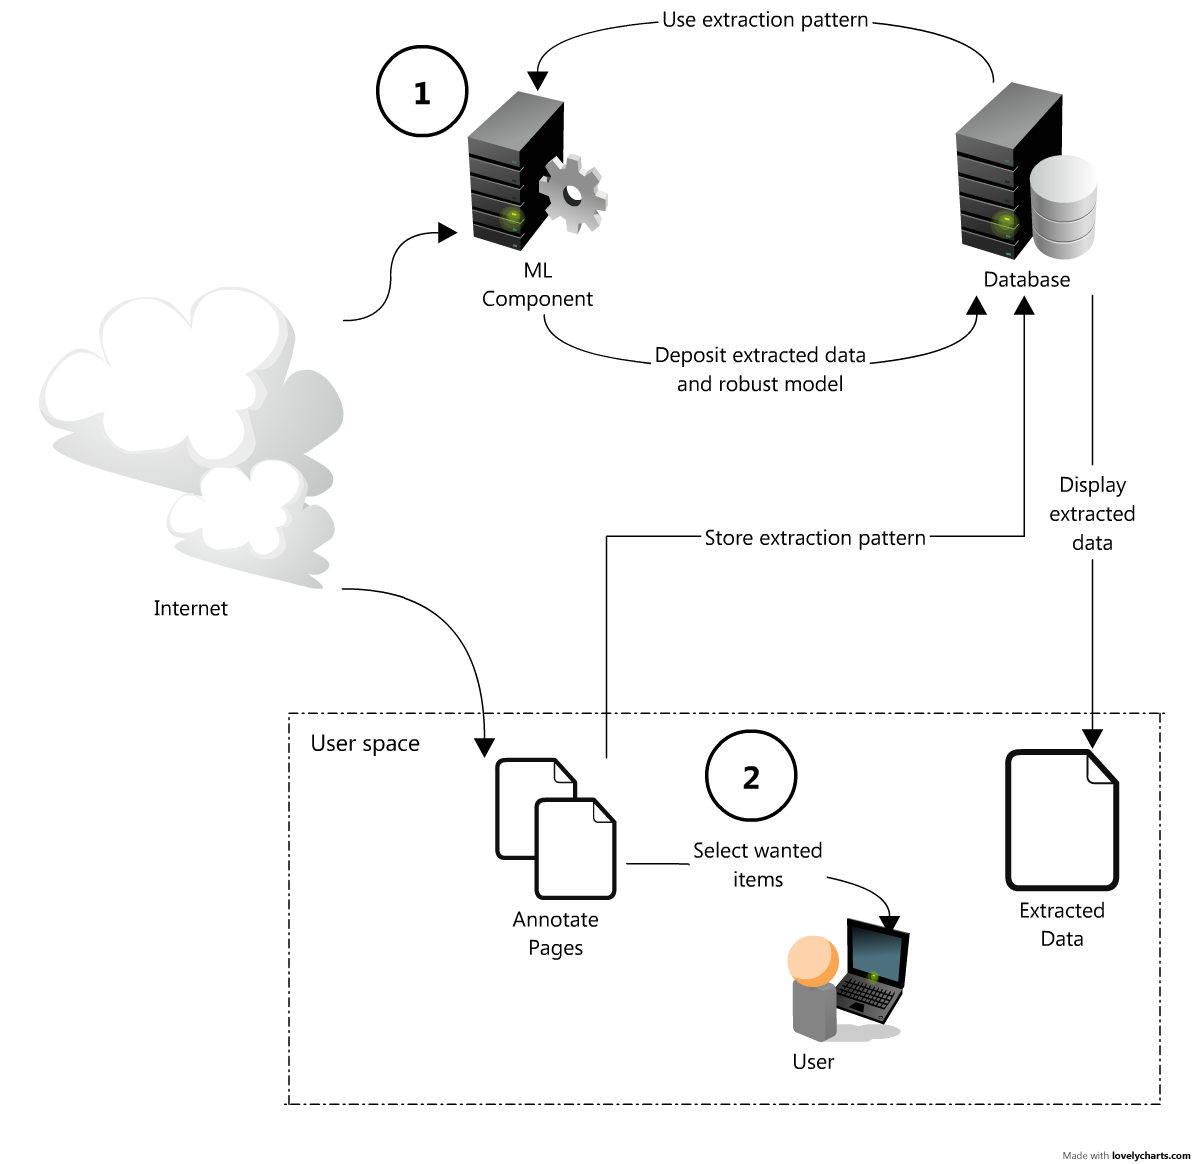
\includegraphics[scale=0.35]{parcels.png} 
\caption{Overview of the system}
\label{fig:architecture}
\end{figure}

Figure \ref{fig:architecture} shows the workflow of the system presented in this report.
% describe figure.. duno what to put.
The section labelled 1 will be described in detail in Chapter \ref{chap:extraction}, and the section labelled 2, which consists of the bookmarklet and user interface, will be described in Chapter \ref{chap:selection}. Both chapters will elaborate on related work, methodology, the sub-system's individual evaluation and analysis of the results.
